\documentclass[10pt,letterpaper]{article}

\usepackage[top=2.5cm,bottom=2.5cm,left=2.5cm,right=2.5cm]{geometry}
\usepackage[utf8]{inputenc}
\usepackage[T1]{fontenc}
\usepackage{lmodern}
\usepackage{setspace}
\usepackage{lineno}
\usepackage{graphicx}
\usepackage{booktabs}
\usepackage{array}
\usepackage{amsmath}
\usepackage{xcolor}
\usepackage[numbers,sort&compress]{natbib}
\usepackage[colorlinks=true,linkcolor=blue,citecolor=blue,urlcolor=blue]{hyperref}

\newcommand{\shorttitle}{Modelo documental en MongoDB para elementos transponibles}

\title{\textbf{Un modelo de datos documental en MongoDB para integrar secuencias, taxonomía y perfiles de k-mers de elementos transponibles a través de reinos}}

\author{
  [Nombre completo del/los autor(es)]\\
  \small Programa de Ingeniería de Sistemas y Telecomunicaciones, Universidad Autónoma de Manizales\\
  \small Curso: Bases de Datos II --- Docente: Simón Gaviria Orrego\\
  \small \texttt{[correo institucional]}
}
\date{}

\begin{document}

\renewcommand{\figurename}{Fig}
\doublespacing
\linenumbers

\maketitle

\begin{abstract}
\noindent
Los elementos transponibles (TEs) ocupan una fracción enorme de los genomas
eucariotas e influyen en la evolución y la regulación génica, pero integrar sus
secuencias, su taxonomía de origen y sus perfiles de composición es un reto de
volumen y de diseño de datos. Presentamos un modelo de datos documental en
MongoDB, implementado con un pipeline en Python, que integra 239{,}946
secuencias de elementos transponibles de 2790 especies (reinos Animalia,
Plantae y Fungi) de la base pública PanTEon, junto con sus perfiles de k-mers
de longitud 1 a 6. El modelo usa dos colecciones --- \texttt{species} y
\texttt{sequences} --- relacionadas por referencia, con los perfiles de k-mers
embebidos como diccionarios dispersos de conteos dentro de cada secuencia. Se
documentan los problemas de calidad de datos encontrados (nombres de especie
inconsistentes, valores faltantes codificados como texto, nombres de clado
usados como "especie"), se resuelven quince consultas y dos preguntas de
investigación propias mediante agregaciones de MongoDB, y se evalúa
experimentalmente el almacenamiento embebido frente a una colección aparte
para los k-mers, midiendo tiempo de carga, espacio en disco y tiempo de
consulta con y sin índice. El almacenamiento embebido resultó entre uno y dos
órdenes de magnitud más rápido en consultas sin índice y operacionalmente más
simple para el patrón de acceso del proyecto, a costa de documentos más
pesados. El código, el modelo y los resultados completos están disponibles en
un repositorio público.
\end{abstract}

\section*{Resumen para el lector no especializado}
\noindent
El ADN de casi todos los seres vivos contiene millones de fragmentos
repetitivos llamados elementos transponibles, capaces de copiarse y moverse
dentro del genoma. Entender cómo se distribuyen estos fragmentos entre especies
de animales, plantas y hongos ayuda a comprender la evolución de los genomas.
En este trabajo organizamos cerca de 240 mil de estos fragmentos, junto con la
información de a qué especie pertenecen y cuál es su "huella digital" química
(la frecuencia con la que aparecen ciertas combinaciones cortas de letras del
ADN), dentro de una base de datos no relacional (MongoDB), pensada para que
investigadores puedan hacer preguntas complejas sobre estos datos de forma
rápida. Documentamos los problemas reales que encontramos en los datos
públicos que usamos, explicamos por qué organizamos la información de una
manera y no de otra, y medimos con datos propios ---no solo intuición--- cuál
estrategia de organización es más conveniente.

\section*{Introducción}

Los elementos transponibles (\emph{transposable elements}, TEs) son secuencias
de ADN capaces de moverse o copiarse dentro de un genoma. Lejos de ser "ADN
basura", ocupan una fracción muy grande de muchos genomas eucariotas --- más
del 80\% en algunas plantas --- y son un motor conocido de evolución, de
regulación génica y de adaptación de las especies. Desde el trabajo seminal de
Wicker et al.~\cite{wicker2007}, los TEs se organizan en una clasificación
jerárquica de tres niveles --- Clase, Orden y Superfamilia --- basada en su
mecanismo de transposición y su estructura. Esta clasificación conceptual es
independiente de la \emph{taxonomía} de la especie en la que se encontró cada
elemento (Reino, Filo, Clase, Orden, Familia, Especie), y ambas jerarquías
comparten nombres de rango (``Clase'', ``Orden'') sin estar relacionadas entre
sí --- una fuente frecuente de confusión al modelar estos datos.

Los grupos de investigación en bioinformática trabajan con \emph{bibliotecas}
de TEs: colecciones de miles de secuencias de muchas especies, generadas tanto
por herramientas automáticas como RepeatModeler2~\cite{flynn2020repeatmodeler2}
como por curación experta en bases de referencia como
Dfam~\cite{storer2021dfam}. Para analizarlas, entrenar clasificadores o
comparar especies, estas secuencias suelen transformarse en \emph{perfiles de
k-mers}: el conteo de cada subsecuencia de longitud $k$ presente en una
secuencia dada. El reto no es solo computar estos perfiles, sino
\textbf{almacenarlos de forma que sigan siendo consultables}: para $k=6$ existen
$4^6=4096$ k-mers posibles por secuencia, y una base con cientos de miles de
secuencias puede generar perfiles para decenas de millones de combinaciones
k-mer/secuencia en total.

En este trabajo diseñamos, implementamos, poblamos, consultamos y evaluamos una
base de datos documental en MongoDB que integra las secuencias, su
clasificación de TE, la taxonomía de su especie de origen y sus perfiles de
k-mers de $k=1$ a $k=6$, a partir de la base pública
PanTEon~\cite{orozco2026panteon,panteon2026zenodo}. El objetivo no es un
hallazgo biológico nuevo, sino demostrar y justificar un conjunto de
decisiones de diseño de datos --- qué se embebe, qué se referencia, cómo se
representan dos jerarquías con nombres de campo que se prestan a confusión, y
cómo se almacenan perfiles de k-mers dispersos de forma eficiente --- y
respaldar esas decisiones con medidas propias de rendimiento y almacenamiento,
no solo con intuición.

\section*{Materiales y métodos}

\subsection*{Datos y problemas de calidad encontrados}

Se usaron las dos fuentes principales de PanTEon Database v1.6.1 (Zenodo,
licencia CC~BY~4.0): un archivo FASTA con 239{,}946 secuencias de elementos
transponibles (encabezado \texttt{>ID\#CLASE/ORDEN/SUPERFAMILIA\ @Especie}) y un
archivo CSV con metadatos taxonómicos de 2790 especies (Kingdom, Phylum, Class,
Order, Family, Species, Source, Source\,2, Notes). Antes de diseñar el modelo
se exploraron ambas fuentes por completo (no por muestreo), lo que permitió
documentar varios problemas de calidad reales:

\begin{itemize}
  \item \textbf{Mayúsculas/minúsculas mezcladas entre secuencias.} Cada
  secuencia individual usa consistentemente mayúscula o minúscula, pero el
  archivo combina ambos estilos entre registros distintos; se normalizó todo a
  mayúsculas al leer.
  \item \textbf{Alfabeto de nucleótidos.} Una vez normalizado el caso, el
  alfabeto observado es estrictamente $\{A,C,G,T,N\}$, sin otros códigos IUPAC
  de ambigüedad. Aproximadamente 35\% de las secuencias (muestra de 20{,}000)
  contienen al menos una N, en promedio $\sim$1.1\% de su longitud en las que
  la tienen, con un caso extremo cercano al 50\%.
  \item \textbf{Valores faltantes codificados como texto.} La columna
  \texttt{Order} del CSV usa, además de valores vacíos, cadenas de texto como
  \texttt{"No trobat"} (catalán, "no encontrado"), \texttt{"No order"},
  \texttt{"Not order identified <Clase>"} o frases con \texttt{"incertae
  sedis"} para representar lo mismo que un valor nulo. Al normalizar estas
  cadenas a \texttt{null}, los nulos de \texttt{Order} pasaron de 29 a 55.
  \item \textbf{Nombres de clado usados como "especie".} 45 filas del CSV
  (todas con \texttt{Source\,=\,Dfam}) tienen en la columna \texttt{Species} un
  taxón superior en vez de un binomio --- por ejemplo \texttt{Primates},
  \texttt{Rodentia} o \texttt{Mammalia} --- correspondientes a bibliotecas de
  consenso ancestral a nivel de clado, no a especies individuales.
  \item \textbf{Cruce FASTA$\leftrightarrow$CSV.} El FASTA y el CSV contienen
  exactamente 2790 especies cada uno, pero 4 no cruzaban directamente por un
  problema de puntuación: el FASTA usa abreviaturas con punto
  (\texttt{subsp.}, \texttt{sp.}) y el CSV las mismas sin punto. Normalizando
  la llave de cruce (quitando puntos, minúsculas, espacios colapsados) las
  2790 especies cruzan exactamente, sin huérfanas en ningún lado.
\end{itemize}

\subsection*{Modelo de datos}

El modelo (Fig~\ref{fig:modelo}) usa dos colecciones principales. \textbf{\texttt{species}}
(2790 documentos) almacena la taxonomía completa de cada especie y la
procedencia de su biblioteca de TEs (\texttt{source}, \texttt{source2},
\texttt{notes}). \textbf{\texttt{sequences}} (239{,}946 documentos) almacena,
por cada elemento transponible: su identificador original (\texttt{original\_id}),
su clasificación de TE (\texttt{te\_class}, \texttt{te\_order},
\texttt{te\_superfamily}), una referencia a su especie (\texttt{species\_id})
más una copia denormalizada de \texttt{species\_name}, la secuencia de
nucleótidos, tres atributos derivados (\texttt{length}, \texttt{gc\_content},
\texttt{n\_percentage}) y los perfiles de k-mers embebidos en
\texttt{kmers.k1}\ldots\texttt{kmers.k6}.

Dos decisiones de diseño merecen justificación explícita:

\textbf{Referencia, no embebido, entre secuencia y especie.} Se consideró
embeber la taxonomía completa en cada secuencia, pero se descartó: la
taxonomía se repetiría en promedio 86 veces por especie
($239{,}946/2790$), y una especie con la corrección de un dato taxonómico
obligaría a actualizar todas sus secuencias. Se referencia por
\texttt{species\_id}, con \texttt{species\_name} denormalizado como única
excepción --- un campo pequeño y estable, necesario para mostrar resultados sin
pagar un \texttt{\$lookup} en cada consulta simple.

\textbf{K-mers embebidos como diccionario disperso, por conteo.} Se almacenan
conteos (no frecuencias, que se derivan dividiendo por $longitud-k+1$) y solo
las combinaciones observadas, no un arreglo denso de $4^k$ posiciones: para
$k=6$ eso implicaría 4096 entradas mayormente en cero por documento. Los
k-mers se embeben junto a su secuencia, no en una colección aparte, porque
nunca se consultan sin ella ni se comparten entre secuencias (ver
\nameref{sec:experimentos} para la comparación cuantitativa con la alternativa).
Los k-mers que contienen cualquier carácter distinto de A/C/G/T se excluyen de
los conteos, no se rellenan ni se tratan como un símbolo adicional del
alfabeto.

Se aplicó validación de esquema (\texttt{\$jsonSchema}) en ambas colecciones
--- campos obligatorios, tipos, y en \texttt{sequences.sequence} un patrón
\texttt{\^{}[ACGTN]+\$} que impide insertar caracteres fuera del alfabeto
esperado --- verificada insertando deliberadamente un documento inválido. Los
índices creados y la consulta que justifica cada uno se listan en la
Tabla~\ref{tab:indices}.

\begin{table}[h]
\centering
\caption{{\bf Índices del modelo de producción.}}
\begin{tabular}{p{3.6cm}p{2.1cm}p{7.8cm}}
\toprule
Índice & Colección & Consulta que soporta \\
\midrule
\texttt{species\_name} (único) & species & Unicidad; cruce por nombre \\
\texttt{match\_key} & species & Cruce FASTA$\leftrightarrow$CSV durante la carga \\
\texttt{kingdom} & species & Agrupar/filtrar por reino \\
\texttt{original\_id} (único) & sequences & Búsqueda por identificador; unicidad \\
\texttt{species\_id} & sequences & \texttt{\$lookup} con species; conteos por especie \\
(\texttt{te\_class}, \texttt{te\_order}, \texttt{te\_superfamily}) & sequences & Conteos por clasificación; filtros de biblioteca \\
\bottomrule
\end{tabular}
\label{tab:indices}
\end{table}

\subsection*{Pipeline en Python}

El pipeline (Python 3.14, \texttt{pymongo}, \texttt{biopython}~\cite{cock2009biopython},
\texttt{pandas}) procesa el FASTA en \emph{streaming} línea por línea (sin
cargarlo completo en memoria, dado su tamaño de $\sim$990~MB), valida cada
encabezado contra el patrón esperado, limpia el CSV conservando solo las nueve
columnas requeridas, normaliza nombres de especie, calcula los perfiles de
k-mers de $k=1$ a $6$ y dos atributos adicionales por secuencia
(\texttt{gc\_content}, \texttt{n\_percentage}), y carga los documentos en
MongoDB con \texttt{bulk\_write} en lotes de 200. La carga completa de las
239{,}946 secuencias tomó 1778.7~s ($\sim$29.6~min) en un equipo de escritorio
estándar, sin omitir ninguna secuencia tras la normalización del cruce
FASTA$\leftrightarrow$CSV. El pipeline es reproducible: cualquier persona
puede regenerar la base desde cero ejecutando tres scripts documentados en el
repositorio sobre los dos archivos descargados de Zenodo.

\subsection*{Diseño de los experimentos}\label{sec:experimentos}

Para evaluar la decisión de embeber los k-mers se comparó esa estrategia
contra una \textbf{colección aparte} (metadatos de la secuencia en una
colección, k-mers en otra, referenciados por \texttt{sequence\_id}), sobre una
muestra aleatoria de 30{,}000 secuencias \emph{ya cargadas} --- es decir, con
los k-mers ya calculados --- para aislar el costo de la estrategia de
almacenamiento del costo de calcular los k-mers. Para cada estrategia se
midió: tiempo de carga (\texttt{bulk\_write}), espacio en disco
(\texttt{collStats}) y el tiempo de tres consultas representativas con y sin
índice (ocultando el índice correspondiente con \texttt{collMod}, usando
\texttt{explain()} para confirmar los documentos examinados).

\section*{Resultados}

\subsection*{Composición de la base}

Tras la carga completa, \texttt{sequences} contiene 239{,}946 documentos y
\texttt{species} 2790, sin IDs duplicados ni referencias
\texttt{species\_id} huérfanas (verificado con una agregación
\texttt{\$group}/\texttt{\$count} y un \texttt{\$lookup} de control). La
Tabla~\ref{tab:composicion} resume la composición por clase y orden de TE
(consulta~1). CLASSI (retrotransposones) domina con 194{,}774 TEs (81.2\%)
frente a 45{,}172 (18.8\%) de CLASSII (transposones de ADN); LTR es el orden
más abundante (119{,}368), seguido de LINE (68{,}382).

\begin{table}[h]
\centering
\caption{{\bf Cantidad de TEs por clase y orden (consulta 1).}}
\begin{tabular}{lrr}
\toprule
Clase & Orden & Cantidad \\
\midrule
CLASSI  & LTR       & 119{,}368 \\
CLASSI  & LINE      & 68{,}382 \\
CLASSII & TIR       & 36{,}471 \\
CLASSII & HELITRON  & 5{,}075 \\
CLASSI  & MITE      & 3{,}456 \\
CLASSI  & SINE      & 3{,}634 \\
CLASSI  & DIRS      & 2{,}933 \\
CLASSI  & PLE       & 344 \\
CLASSII & CRYPTON   & 112 \\
CLASSII & RETROPOSON& 113 \\
CLASSII & MAVERICK  & 58 \\
\midrule
\textbf{Total CLASSI}  & & \textbf{194{,}774} \\
\textbf{Total CLASSII} & & \textbf{45{,}172} \\
\bottomrule
\end{tabular}
\label{tab:composicion}
\end{table}

Entre reinos (consulta~3), Animalia está dominado por LINE (44{,}477 TEs)
sobre LTR (25{,}382), mientras que Plantae y Fungi están dominados por LTR ---
visible de un vistazo en la Fig~\ref{fig:comp-reino}, que agrega los 11
órdenes para los 3 reinos a partir de una agregación con \texttt{\$lookup}.
Las 10 especies con más TEs están encabezadas por \emph{Malus domestica}
(1627), \emph{Danio rerio} (1352) y \emph{Callithrix jacchus} (1294)
(consulta~4); en el otro extremo, varias decenas de especies tienen
exactamente 1 TE registrado, consistente con bibliotecas de anotación
preliminar más que con genomas realmente pobres en TEs.

\begin{figure}[h]
\centering
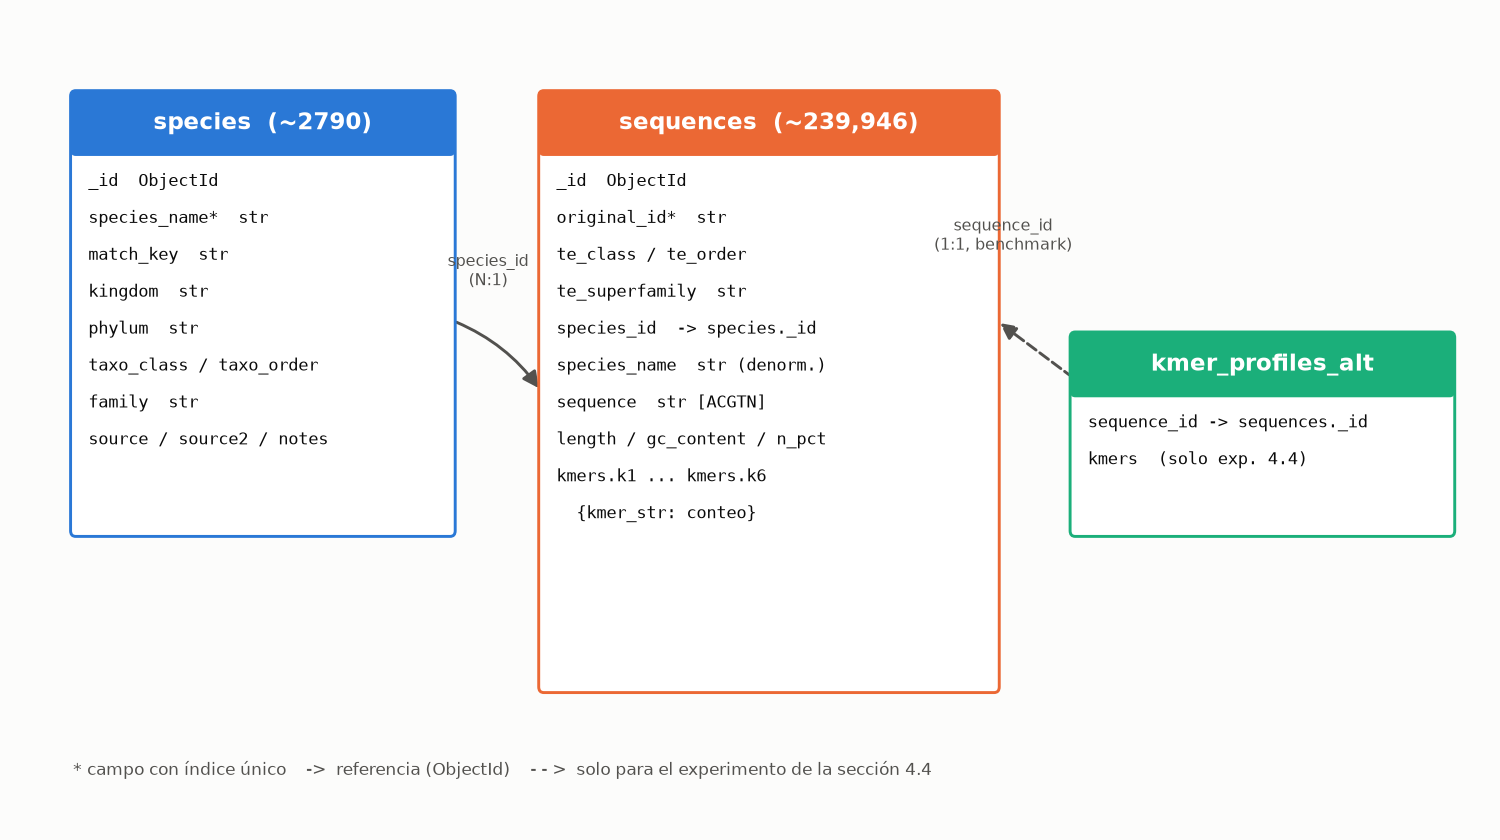
\includegraphics[width=0.85\textwidth]{figures/fig0_modelo_datos.png}
\caption{{\bf Modelo de datos.} Dos colecciones de producción
(\texttt{species}, \texttt{sequences}) relacionadas por referencia, y una
colección auxiliar (\texttt{kmer\_profiles\_alt}) usada solo en el experimento
de la sección de Materiales y métodos.}
\label{fig:modelo}
\end{figure}

\begin{figure}[h]
\centering
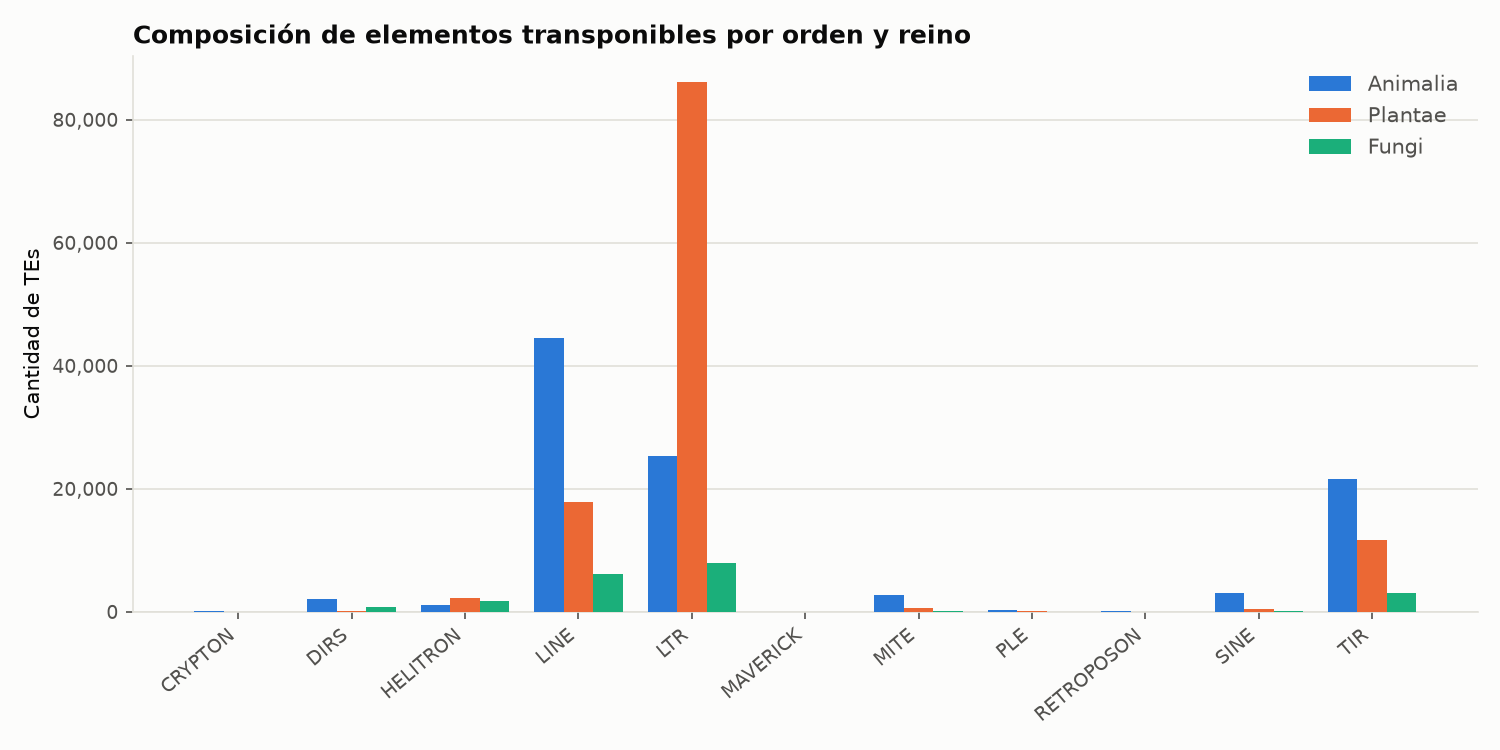
\includegraphics[width=0.95\textwidth]{figures/fig1_composicion_por_reino.png}
\caption{{\bf Composición de elementos transponibles por orden y reino.}
Cantidad absoluta de TEs de cada orden en Animalia, Plantae y Fungi, calculada
con una agregación \texttt{\$lookup} + \texttt{\$group} sobre las 239{,}946
secuencias.}
\label{fig:comp-reino}
\end{figure}

\subsection*{Longitud y contenido GC}

CLASSI es, en promedio, más del doble de largo que CLASSII (4453.1~nt frente a
2137.3~nt; consulta~5), con longitud mínima de 81~nt y máxima de 19{,}926~nt
en toda la base. La Fig~\ref{fig:longitud} muestra la distribución completa
por orden: MAVERICK y LTR tienen la mediana más alta y la mayor dispersión,
mientras que SINE y MITE son consistentemente cortos. El contenido GC
promedio (consulta~6) es más alto en Fungi (46.2\%) y más bajo en Plantae
(41.2\%) (Fig~\ref{fig:gc}); entre órdenes, SINE y DIRS tienen el GC\% más
alto ($\sim$53\%) y TIR/MAVERICK el más bajo ($\sim$40\%). El TE más largo de
toda la base (19{,}926~nt, orden LTR/GYPSY) pertenece a \emph{Helianthus
annuus}; los más cortos (81--100~nt) aparecen en los tres reinos (consulta~7).

\begin{figure}[h]
\centering
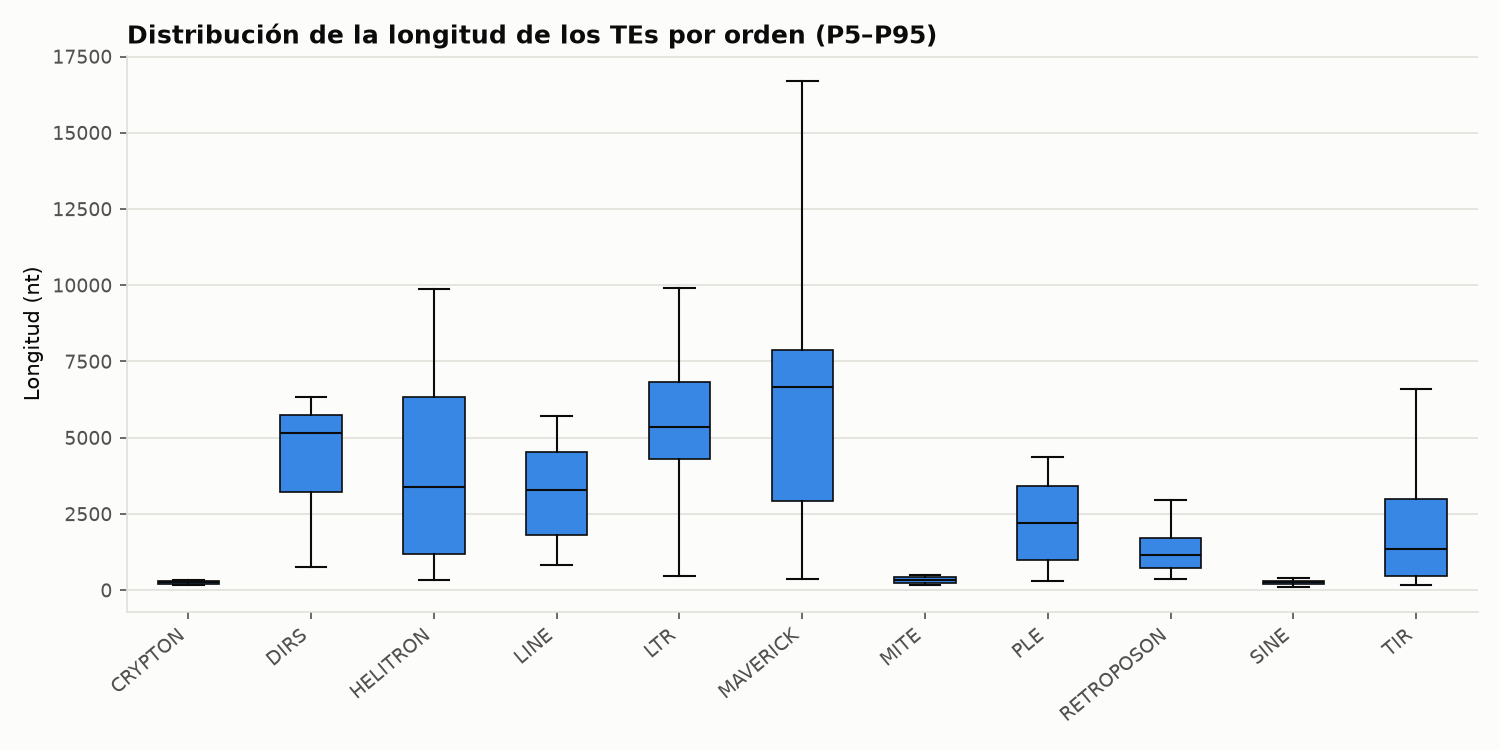
\includegraphics[width=0.95\textwidth]{figures/fig2_longitud_por_orden.png}
\caption{{\bf Distribución de la longitud de los TEs por orden.} Cajas
construidas con cuartiles calculados en MongoDB (\texttt{\$percentile},
P5--P95), sin necesidad de extraer los datos crudos.}
\label{fig:longitud}
\end{figure}

\begin{figure}[h]
\centering
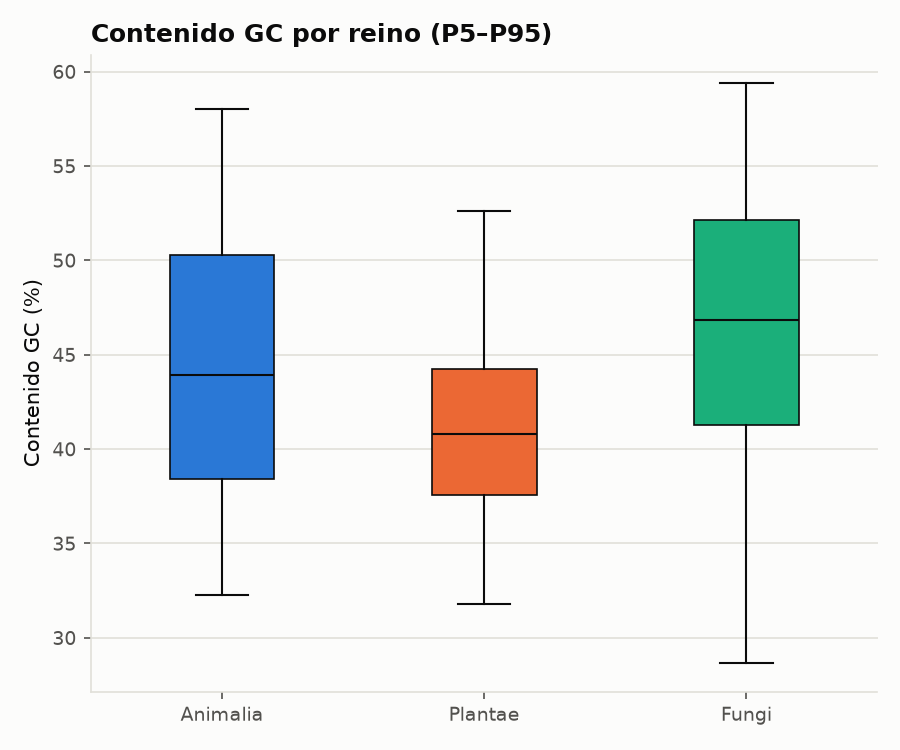
\includegraphics[width=0.6\textwidth]{figures/fig3_gc_por_reino.png}
\caption{{\bf Contenido GC por reino (P5--P95).}}
\label{fig:gc}
\end{figure}

\subsection*{Origen de los datos y control de calidad}

Agrupando por la columna \texttt{Source} del CSV (consulta~13), las
bibliotecas generadas automáticamente con RepeatModeler2 + MCHelper
(\texttt{RM2+MCH}) cubren 2404 especies con 208{,}354 secuencias (86.7
secuencias/especie en promedio, longitud media 4375.5~nt), mientras que las
bibliotecas de referencia Dfam cubren 386 especies con 31{,}592 secuencias
(81.8 secuencias/especie, longitud media 1653.8~nt) --- una diferencia de
longitud notable, consistente con que Dfam incluye más fragmentos de consenso
cortos y las 45 bibliotecas de clado ancestral descritas en Métodos. Como
consulta de control de calidad propia (consulta~14), se identificaron 4374
secuencias (1.82\% del total) con más de 5\% de contenido N, posible indicio
de regiones de ensamblaje genómico incompleto; estas secuencias se conservan
en la base (no se descartan), y el pipeline simplemente excluye de los
conteos cualquier k-mer que contenga una N.

\subsection*{Patrones de k-mers}

La Fig~\ref{fig:heatmap} muestra la frecuencia relativa promedio de los 16
2-mers para cada orden de TE (consulta propia, visualización~4). Casi todos
los órdenes comparten el mismo patrón dominante --- AA/TT/AT altos, CG
consistentemente el más bajo, el conocido déficit de dinucleótidos CpG de los
genomas eucariotas --- mientras que RETROPOSON y SINE se distinguen por tener
CC y GG relativamente más altos que el resto. Recuperar el perfil completo de
k-mers de una secuencia dada para un $k$ dado (consulta~15) es una búsqueda
puntual por \texttt{original\_id} seguida de una proyección de
\texttt{kmers.k\{k\}}; para \texttt{PDB00000001} (HELITRON de
\emph{Halicephalobus\ mephisto}, el ejemplo del enunciado del taller, recuperado
en la consulta~8 junto con su taxonomía completa vía \texttt{\$lookup}) el
perfil de 2-mers tiene presentes las 16 combinaciones posibles, con AA (306) y
TT (234) como las más frecuentes.

\begin{figure}[h]
\centering
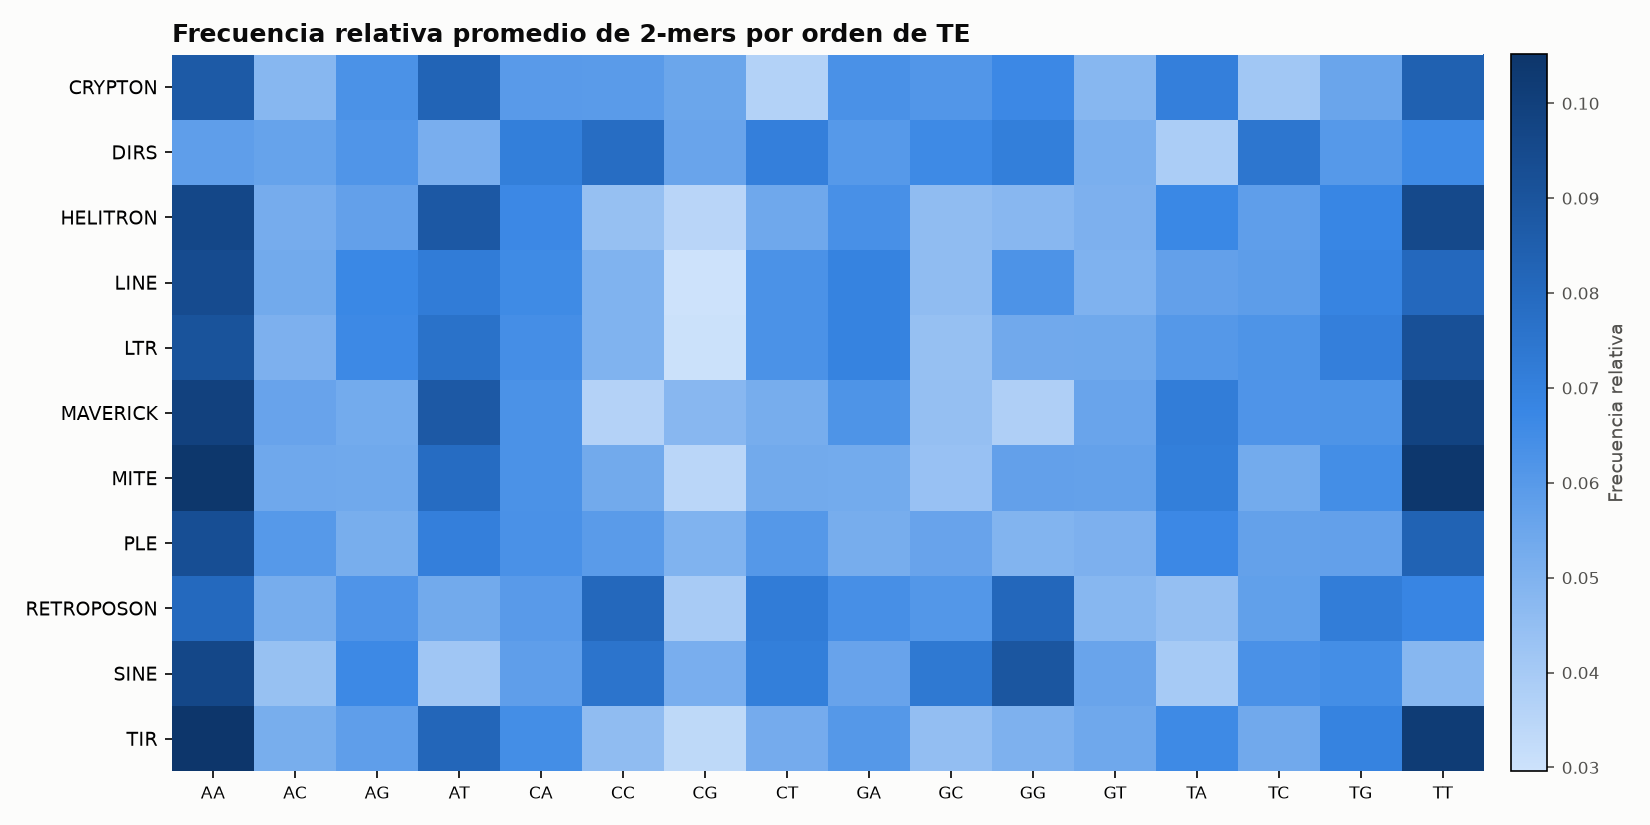
\includegraphics[width=0.95\textwidth]{figures/fig4_heatmap_kmers2.png}
\caption{{\bf Frecuencia relativa promedio de 2-mers por orden de TE.} Cada
celda es el promedio, sobre todas las secuencias de ese orden, del conteo de
un dinucleótido dividido entre el total de 2-mers de la secuencia.}
\label{fig:heatmap}
\end{figure}

\subsection*{Evaluación experimental: embebido frente a colección aparte}\label{sec:resultados-exp}

Sobre la muestra de 30{,}000 secuencias, el espacio en disco total fue similar
entre ambas estrategias (509.1~MB embebido frente a 499.6~MB en colección
aparte, Tabla~\ref{tab:benchmark}) porque en ambas la secuencia de nucleótidos
--- el campo más pesado --- se guarda una sola vez. La diferencia decisiva
aparece en las consultas \textbf{sin índice}: escanear la colección embebida
(documentos grandes, con la secuencia completa y los 6 perfiles de k-mers)
para encontrar una secuencia por su \texttt{original\_id} tomó 3.15~s,
examinando los 30{,}000 documentos; la misma búsqueda sobre la colección
aparte (documentos pequeños, solo k-mers) tomó 0.035~s --- casi 90 veces más
rápido. \textbf{Con índice}, ambas estrategias resuelven la búsqueda puntual en
1--2~ms examinando un solo documento, por lo que esta diferencia desaparece
en el modelo de producción (que sí tiene el índice sobre \texttt{original\_id}).

\begin{table}[h]
\centering
\caption{{\bf Comparación embebido vs. colección aparte (muestra de 30{,}000 secuencias).}}
\begin{tabular}{lrr}
\toprule
Métrica & Embebido & Colección aparte \\
\midrule
Tiempo de carga (s) & 14.65 & 20.52 \\
Espacio en disco (MB) & 509.12 & 499.62 (66.16 + 433.46) \\
Índices (MB) & 0.77 & 1.82 \\
Búsqueda puntual, con índice (s) & 0.00239 & 0.00163 \\
Búsqueda puntual, sin índice (s) & 3.15198 & 0.03458 \\
Suma global de un k-mer, agregación (s) & 0.45263 & 0.33266 \\
Metadatos + k-mers de una secuencia (s) & 0.00170 (1 consulta) & 0.00112 (2 consultas) \\
\bottomrule
\end{tabular}
\label{tab:benchmark}
\end{table}

Para el caso de uso combinado --- traer los metadatos de una secuencia junto
con su perfil de k-mers, el patrón de acceso más común del proyecto --- el
modelo embebido lo resuelve con una sola consulta, mientras que la colección
aparte necesita dos consultas secuenciales; a esta escala la diferencia de
tiempo medida fue pequeña e incluso ligeramente favorable a la colección
aparte en términos de latencia bruta, pero a costa de duplicar la complejidad
operacional del código cliente.

\section*{Discusión}

Los resultados respaldan la decisión de diseño de embeber los k-mers junto a
su secuencia: dado que nunca se consultan de forma aislada ni se comparten
entre secuencias, una colección aparte solo añade una referencia y un segundo
\emph{round-trip} sin beneficio claro para este patrón de acceso, y con el
índice correcto el costo de documentos más pesados queda completamente
mitigado. La colección aparte solo mostraría ventaja real en un escenario
distinto al de este proyecto: un servicio que escanea o agrega k-mers con
mucha frecuencia \emph{sin} tocar nunca la secuencia completa, donde evitar
cargar ese campo en cada documento leído ahorraría E/S de forma sistemática.
Este hallazgo generaliza una intuición común en el modelado de documentos
--- "lo que se lee junto, se guarda junto" --- con una medida concreta de cuánto
cuesta no seguirla quando no hay índice de apoyo (90$\times$ en este caso).

La exploración de calidad de datos fue, en sí misma, una parte sustancial del
trabajo de diseño. Los valores faltantes codificados como texto libre en
distintos idiomas (catalán e inglés mezclados en la misma columna) y el uso
de nombres de clado como si fueran nombres de especie son el tipo de
inconsistencia que un modelo relacional con tipos estrictos habría forzado a
resolver antes de poder cargar los datos; en un modelo documental sin
\texttt{\$jsonSchema} estricto en todos los campos, estos problemas pueden
pasar desapercibidos silenciosamente. Aplicar validación de esquema solo en
los campos verdaderamente estructurales (identificadores, secuencia, tipos
numéricos) --- y dejar los campos taxonómicos más flexibles (\texttt{string}
o \texttt{null}) --- fue un compromiso deliberado entre seguridad de datos y
la naturaleza real, incompleta, de los metadatos taxonómicos disponibles.

\textbf{Limitaciones.} El experimento de almacenamiento se corrió sobre una
muestra de 30{,}000 secuencias (12.5\% de la base), no sobre las 239{,}946
completas, por restricciones de tiempo; aunque no hay razón para esperar que
la proporción cambie cualitativamente a mayor escala, una validación sobre la
base completa sería el siguiente paso natural. El umbral de 5\% de contenido N
usado en el control de calidad es una elección heurística propia, no un
estándar de la literatura. Finalmente, el cruce de especies se resolvió por
normalización de texto (minúsculas, sin puntos); una especie con un error
ortográfico genuino en una sola fuente no sería detectada por este método y
quedaría, silenciosamente, sin cruzar.

\textbf{Si los datos crecieran 10 o 100 veces}, el diseño actual seguiría
siendo válido en su estructura, pero dos decisiones deberían revisitarse: (1)
el cálculo de k-mers en Python puro (sin paralelismo) tardó cerca de 30
minutos para 240 mil secuencias; a 24 millones de secuencias ese tiempo sería
inviable sin paralelizar el pipeline o delegar el cómputo a una extensión
nativa; y (2) aunque el experimento de la sección de Resultados no encontró
ventaja de la colección aparte para k-mers, a una escala donde la colección
\texttt{sequences} no quepa cómodamente en el conjunto de trabajo en memoria
de MongoDB, separar el campo más pesado (la secuencia) de los campos
consultados con más frecuencia podría volver a ser ventajoso --- una pregunta
que este experimento, a la escala actual, no puede responder por sí solo.

\section*{Conclusiones}

Se diseñó, implementó y evaluó un modelo de datos documental en MongoDB que
integra 239{,}946 secuencias de elementos transponibles, su taxonomía y sus
perfiles de k-mers de $k=1$ a $6$, resolviendo las quince consultas
obligatorias y dos preguntas de investigación propias mediante agregaciones.
La decisión de embeber los k-mers junto a su secuencia, en vez de separarlos
en una colección aparte, se justificó no solo conceptualmente sino con una
medida experimental propia: con el índice adecuado ambas estrategias rinden
igual, y sin él la estrategia embebida es hasta 90 veces más lenta en
búsquedas puntuales --- evidencia directa de que el índice sobre
\texttt{original\_id}, y no la separación en colecciones, es lo que realmente
sostiene el rendimiento de este modelo. La exploración sistemática de ambas
fuentes de datos, antes de fijar el esquema, permitió documentar y resolver
problemas de calidad reales (nombres inconsistentes, valores faltantes
disfrazados de texto, nombres de clado usados como especie) que de otro modo
habrían quedado embebidos silenciosamente en el modelo final.

\section*{Disponibilidad de datos y código}

El código completo del pipeline, el modelo de datos, las consultas, los
experimentos y las figuras está disponible en un repositorio público:
\url{https://github.com/JuanGomez507/panteon-bd2-elementos-transponibles}. Los
datos originales (FASTA y CSV) provienen de PanTEon Database
v1.6.1~\cite{panteon2026zenodo}, disponible en Zenodo bajo licencia CC~BY~4.0;
el repositorio del proyecto no redistribuye estos archivos --- documenta cómo
descargarlos y reconstruir la base desde cero de forma reproducible.

\section*{Agradecimientos}

A los autores de PanTEon Database por hacer públicos los datos que hicieron
posible este trabajo.

\bibliographystyle{unsrtnat}
\bibliography{references}

\end{document}
